\chapter{Blockchain: A Practical Overview and Use Cases}\label{blockchain}

\begin{quote} 
  \emph{This Chapter presents a more technical overview of the Blockchain
  technology. A more in-depth exploration of the Ethereum and Hyperledger
  Fabric platform characteristics is also shown. Smart contracts and use cases
  of this technology in Healthcare are also shown.}
\end{quote}

As discussed in Chapter~\ref{background}, Blockchain implementations are an
emerging structure for distributed computing systems that provide an immutable
history of records written to a ledger, even when there is no implicit trust
relationship between the parties involved~\cite{Barclay2017}. The origin of
this technology can be traced back to the realization that full centralization
should be avoided in critical services.

\section{Trust in a Network}

Banks used to keep track of their financial transactions by writing on a book
usually located at the central bank. This book was often called ledger.
Whenever a transaction occurred someone wrote the record of the transaction on
the book, permanently adding information to the book. In short, the ledger acts
as a permanent mean of storing all the transaction details between the bank and
other entities. 

Nowadays, banks do not use the ledger in a book format. Instead, the ledger is
the structure that holds all transaction information the bank possesses. It is
a structure that keeps the original purpose of recording all the transactions
that are made.

Imagine the following situation, Bob is on vacation and needs to borrow money
from Alice, his wife. Bob calls Alice to ask for some money and Alice tells him
it will send the money right away. Jane then proceeds to use her homebanking
system to transfer some of her money to Bob. Finally Alice calls Bob to tell
him that she made the request to send money to him.  As seen on
Figure~\ref{fig:centralizedvsdescentralized} Bob and Alice need to use and
trust the the bank as a middle man in order to complete this transaction. If
the bank was ever to be unavailable, the bank's database was corrupted or if
someone with  privileged access was able to intercept the transactions from
inside the bank then all transactions between Bob and Alice would fail creating
additional costs to all parties involved. 

\begin{figure}[h]
  \centering
  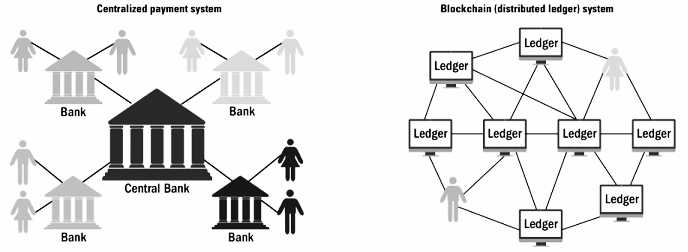
\includegraphics[width=1\linewidth]{imgs/blockchainvscentralizedNetwork.png}
  \caption{\label{fig:centralizedvsdescentralized} A comparison between a
  Centralized Banking System and a Distributed Ledger.
  (Source:~\href{https://www.imf.org/external/pubs/ft/fandd/}{Finance \&
  Development}, 2016)}
\end{figure}

For a long time it was necessary, to establish trust between two entities, a
middle-man with a neutral stake. While the ledger is also at the core of the
Blockchain, this technology aims to solve the dependency placed upon third
parties using decentralization and aims to make two different entities trust
each other through constant replication of the ledger, a security mechanism
called consensus.

For example, in the Bitcoin's Blockchain case, Alice initializes this process
in the Blockchain by signing a transaction that describes some of her money is
being sent to Bob's digital wallet address. The transaction is placed in a pool
of unconfirmed transactions and broadcasted to every node. Every 10 minutes a
miner~\footnote{Bitcoin miners help keep the Bitcoin network secure by
approving transactions and then writing in the Blockchain ledger. In a
Proof-of-Work consensus based Blockchain, like Bitcoin, miners use special
software and hardware to solve complex mathematical problems and are issued a
certain number of Bitcoins in exchange, if a solution is found, as an incentive
to mining.} solves a hash\footnote{A cryptographic hash function allows one to
easily verify that some input data maps to a given hash value. However, if the
input data is unknown, it is deliberately difficult to reconstruct it by
knowing the stored hash value. The cryptograhic puzzle that miners need to
solve is to find an input value, often called nonce, that produces an output
hash value that satisfies a defined condition by the mining software.} problem,
collects some of these unconfirmed transactions, packages them in a block and
broadcasts that he found the solution. The output of the hash function is
easily verified, and every miner confirms if the block is considered valid. If
consensus is reached by the nodes, the block is added to the Blockchain
(written in the ledger) and the new state is persisted on all peers through
replication of the ledger. At this point the transaction is confirmed,
requiring no middle man to ensure the transaction is trustworthy and valid. The
transaction authentication process is shown on
Figure~\ref{fig:bitcoinTransaction}

\begin{figure}[h]
	\centering
	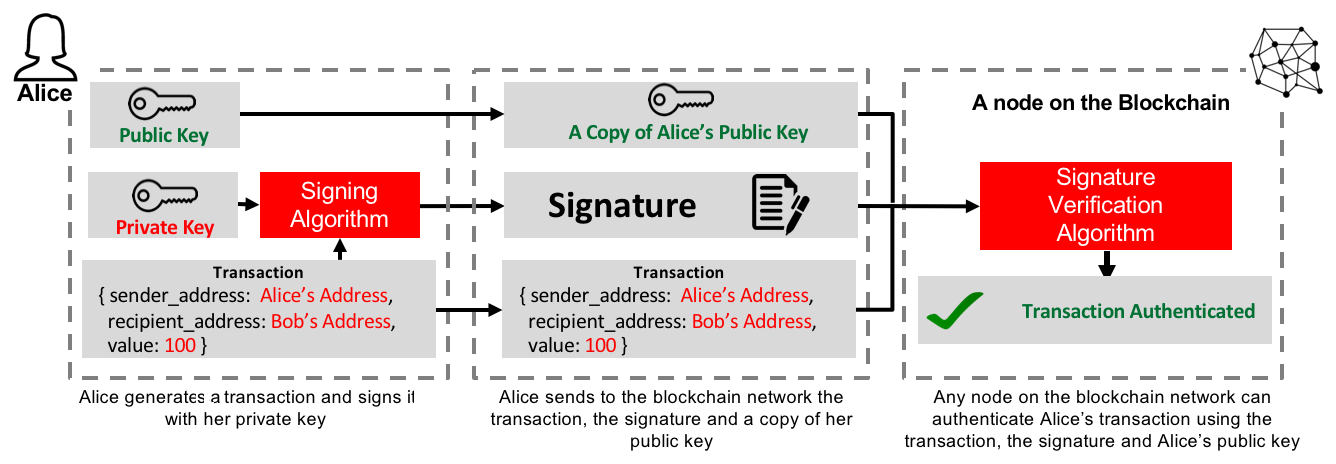
\includegraphics[width=1\linewidth]{imgs/bitcoinTransaction.png}
  \caption{\label{fig:bitcoinTransaction} Bitcoin Transaction Authentication
  Process
  (Source:~\href{http://adilmoujahid.com/images/blockchain-public-crypto.png}{Adil
  Moujahid}, 2018)}
\end{figure}

While consensus has a system performance impact due to the necessary
replication of data and wasteful energy and computing power in the mining
process, it is a mechanism that establishes a set of rules that defines if a
sequence of transactions is considered valid.  Different Blockchain
implementations often use a variety of consensus protocols to balance this
trade-off.

\section{Permissionless and Permissioned Blockchain Implementations}

There are three types of computer systems, as seen on Figure
\ref{fig:typesofnetworks}.

\begin{figure}[h]
	\centering
	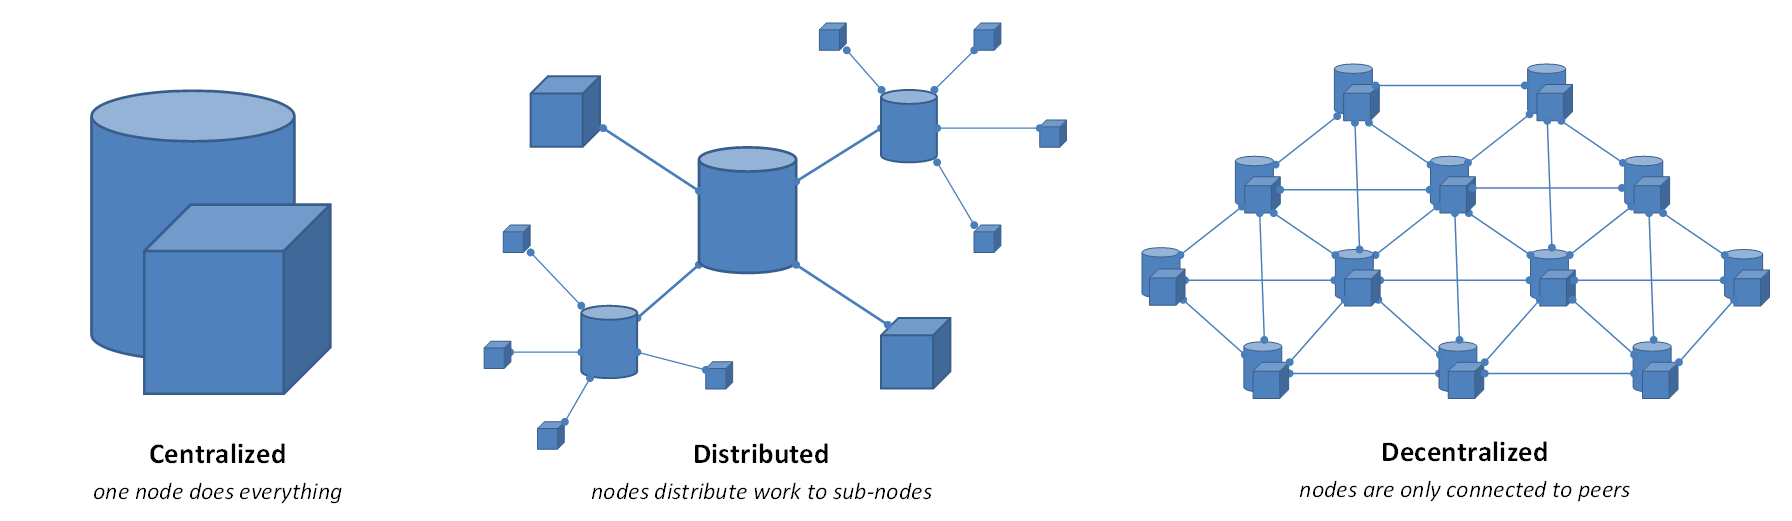
\includegraphics[width=1\linewidth]{imgs/typesofnetworks.png}
  \caption{\label{fig:typesofnetworks} A comparison between different types of
  computing systems. (Source: Eric Grange, 2016)}
\end{figure}

Put simply, a centralized system is one that is governed by a hierarchical
authority, for example, banks and credit card companies. If you want to use a
Visa card you must request access from Visa and be approved. At any time your
access to that line of credit and your funds may be made unavailable to you and
your access permanently revoked~\cite{Dreifuerst2018}.

In contrast, distributed systems are based upon the philosophy that processing
is shared across multiple nodes even if the decisions themselves may still be
centralized and use complete system state knowledge of the network. Finally, a
decentralized system is one where no single node can make a decision
individually, instead relying on the other participants to reach an agreement
and make a decision, as no single node has a complete system state knowledge.
With this in mind, a decentralized system is seen as a subset of a distributed
system.

A Blockchain is a distributed by design. However there are two major
implementation categories as discussed briefly on Chapter~\ref{background}.

Permisionless Blockchain implementations were the first to appear and while
some industries saw benefits in using the technology, some saw drawbacks to
adopting it in enterprise-grade systems~\cite{Gopinath2016} due to this
unregulated nature. They do have some advantages however compared to
traditional systems.

\textbf{Permisionless} Blockchain implementations, like the Bitcoin's and
Ethereum's Blockchain for example, have no barrier to entry. This means that
anyone can, in theory, participate in the network, write into it as a result of
mining and store data in the ledger sharing the work needed to maintain the
network.  Permisionless implementations have some strengths. These are
completely open and transactions are transparent while also being able to offer
anonymity or pseudo-anonymity. They also take away the need for system
administrators or central servers since the network is based exclusively on
peer-to-peer technology and decisions are made by every participant, creating
reduced costs to maintain and deploy Decentralized applications. On the other
hand, these implementations are slower than traditional systems because every
node must participate in consensus creating an overhead before a transaction is
considered verified. Due to this there is also a time cost associated because
of the need to wait until verification of the transaction. They operate without
clear legal rules and are trust-free, meaning that there is no responsible
entity if data loss or damages affect systems based on this implementation.

\textbf{Permissioned} Blockchain implementations have some clear advantages for
enterprise. They are faster because consensus is done by a set of nodes instead
of the entire network, can fall back on the legal system because it features an
identity service. This means the platform is auditable and that there is a
legal responsible entity or entities that manage the network. However, when
compared to the permissionless variant, costs are higher due to having the need
for a system administrator and servers to manage the network, featuring a
private membership meaning that they are closed to the general public and
managed by a set of entities and are a compromise between the original vision
of a completely decentralized network and enterprise needs and concerns. 

Enterprises benefit greatly from the immutability of the Blockchain
architecture, in that all records cannot be changed. By adding authorized
identity services onto Blockchain, they can meet the regulatory needs of their
industries, by allowing the network to be auditable and assets to be traceable,
falling back to laws or regulations if a dispute between participating entities
occurs~\cite{Barclay2017}.

\section{A Decentralized Open Platform - Ethereum} \label{ethereumPlatform}

Ethereum is a permissionless Blockchain implementation. It is a platform that
lets anyone build and use decentralized applications commonly named Ðapps. It
is an open-source project developed primarily by the Ethereum Foundation and
was designed to be adaptable and flexible, in contrast to Bitcoin's Blockchain
that only records financial transactions~\cite{EthereumDocs2018}, as discussed
in Section~\ref{blockchainasaPlatform}.

It features a friendly programming language called Solidity that is influenced
by C++, Python and Javascript. It is designed to allow an easy way for
developers to create new applications on the Ethereum platform with code of
arbitrary algorithmic complexity in a turing complete language. Smart Contract
application code targets the Ethereum Virtual Machine (EVM), presented shortly,
and is then deployed to the Blockchain via a local Ethereum
node~\cite{Wood2017,Barclay2017}.

At the heart of Ethereum is the Ethereum Virtual Machine, as seen on
Figure~\ref{fig:evm}. Ethereum also includes a peer-to-peer network protocol,
as does any Blockchain. The Ethereum Blockchain database is maintained and
updated by many nodes connected to the network. Each and every node of the
network runs the EVM and executes the same instructions in order to maintain
consensus across the entire Blockchain. Decentralized consensus gives Ethereum
a high degree of fault tolerance, ensures zero downtime, and makes data stored
on the Blockchain forever unchangeable and
censorship-resistant~\cite{EthereumDocs2018}.

\begin{figure}[h]
  \centering
  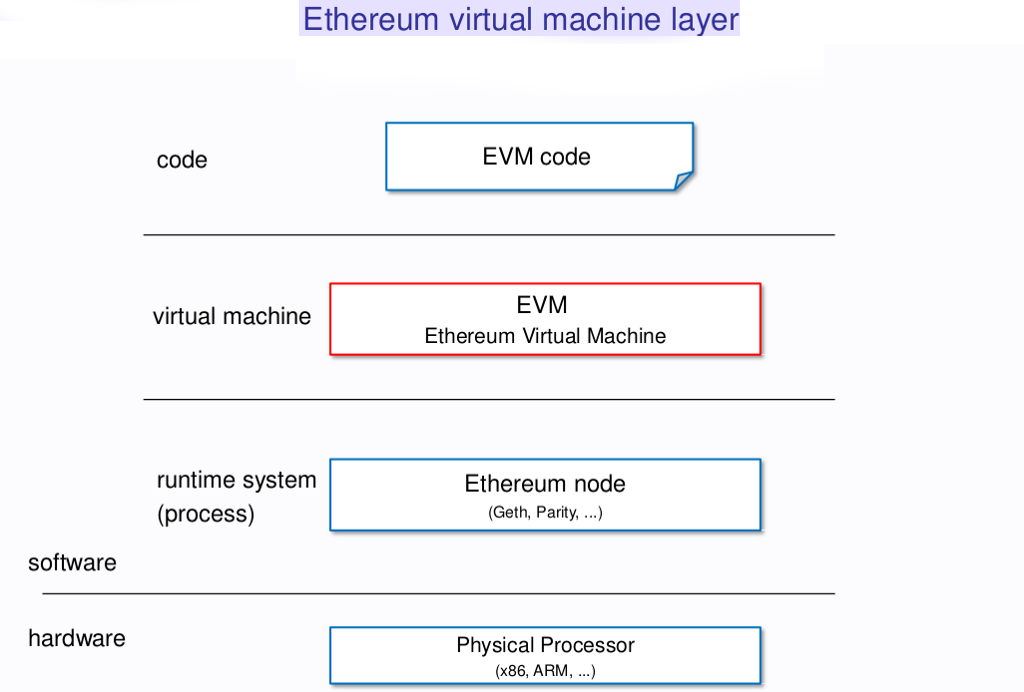
\includegraphics[width=1\linewidth]{imgs/ethereumVirtualMachine.png}
  \caption{\label{fig:evm} A diagram of where the Ethereum Virtual Machine fits
  into the Ethereum Platform (Original: Vaibhav Saini, 2018)}
\end{figure}

Users must pay a small transaction fee to the network each time they execute a
transaction. This protects the Ethereum Blockchain from frivolous or malicious
computational tasks, like Distributed Denial of Service attacks or an infinite
loop in smart contract logic. The sender of a transaction must pay for each
step of the “program” they activated, including computation and memory storage.
These fees are paid in amounts of Ethereum’s native value-token, ether, and
then these transaction fees are collected by the nodes that validate the
network commonly called miners. Miners are nodes in the network that receive,
propagate, verify, and execute transactions. Ethereum currently uses a
Proof-of-Work based consensus algorithm but plans to change to a Proof-of-Stake
based algorithm due to environmental and financial concerns as well as reduced
centralization risks~\cite{EthereumDocs2018,EthereumPOSFAQ2018}.

Ethereum has a live production network called “mainnet” available for any
developer to deploy applications to, as well as three test networks. "Ropsten”
is based on a Proof-of-Work algorithm while "Rinkeby" and "Kovan" are based on
Proof of Authority~\footnote{In Proof of Authority based networks, transactions
and blocks are validated by approved accounts, known as validators. Validators
run software allowing them to put transactions in blocks. The process is
automated and does not require validators to be constantly monitoring their
computers. It does, however, require maintaining the authority node
uncompromised.}. All of these are publicly available and free to
use~\cite{Barclay2017,EthereumTestNetworks2018}.

Ethereum has had some unforeseen problems along the way, namely the Digital
Decentralized Autonomous Organization heist where a hacker took advantage of a
bug in a smart contract to steal a great sum of money requiring a hard fork of
the network to a point before the incident~\cite{Leising2017}. Also, with
Ethereum frequently reaching full transaction capacity, scaling solutions are
the next big investment and focus~\cite{ethereumScalability2018}.

There are a few proposed solutions by Buterin. For example, \textbf{sharding}
is a solution that aims to avoid every node processing all data in order to
verify and process a transaction. When transactions are initiated they will not
be directed to all the nodes but would instead only be directed to those
depending on the shard in question.  Another solution is \textbf{off chain
computation} where a layer apart from the Blockchain is created and where all
the computation or solving of a complex mathematical equation takes place. This
would not only take the load off the Ethereum Blockchain but also help decrease
the cost of transaction verification and processing. This mechanism would
ensure that the tasks that account for slower transaction speeds on the
Ethereum’s Blockchain do not affect the whole network. Finally, to avoid every
node having the need to download the entirety of the Blockchain's data, the
complete picture can be stored on cloud and each node only has to store and
load relevant data~\cite{ethereumBlogScalability2018}.

\section{A Permissioned Distributed Ledger Platform - Hyperledger Fabric}
\label{distributedLedgerPlatform}

As discussed in Section~\ref{enterpriseBlockchain}, Hyperledger Fabric is a
platform for distributed ledger solutions featuring a modular architecture. It
provides developers with a permissioned platform targeted at business and
enterprise use cases that supports pluggable implementations of different
components to accommodate the complexity and intricacies that exist across the
economic ecosystem. It is an open source project initially commited by IBM  and
estabilished under the Linux Foundation, being developed by over 44
organizations and more than 250
members~\cite{HyperledgerFabricDocs2017,HyperledgerGrowth2018}.

It supports the creation of smart contracts, \textbf{commonly called chaincode
in Fabric}, that are authored in general-purpose programming languages such as
Java, Go and Node.js rather than constrained domain specific languages. 

Chaincode in Fabric consists of two components. The \textbf{code itself}, which
describes the logic of the program running in the execution phase, and the
\textbf{endorsement policy} that describes how a specific chaincode transaction
is validated. For example, a typical endorsement policy lets the chaincode
specify the endorsers for a transaction in the form of a set of peers that are
necessary for endorsement and subsequent successful
validation~\cite{Androulaki2018}. Chaincode runs in a container isolated from
the peer process which consented its installation providing aditional control
over information dissemination.

At the heart of Fabric is the permissioned distributed ledger that provides a
way to secure the interactions among a group of entities that have a common
goal but which may not fully trust each other. By relying on the identities of
the participants, a permissioned ledger platform can use a more traditional
Crash Fault Tolerant or Byzantine Fault Tolerant consensus protocols that do
not require mining or an associated currency in order to achieve consensus.

\begin{figure}[h]
  \centering
  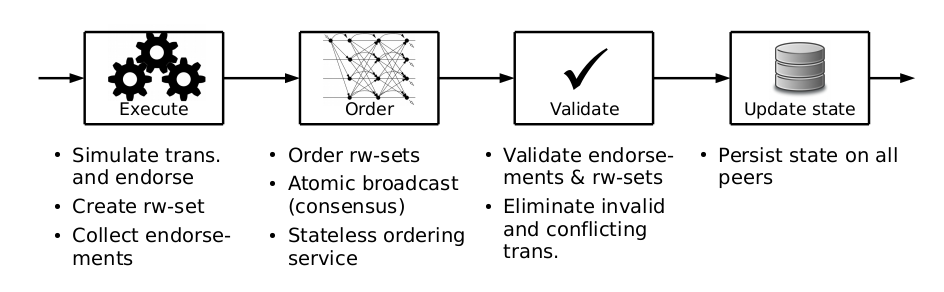
\includegraphics[width=1\linewidth]{imgs/executeOrderValidate.png}
  \caption{\label{fig:executeorder} Execute-order-validate architecture of
  Fabric (Source: IBM, 2018)}
\end{figure}

Fabric introduces the execute-order-validate Blockchain architecture as shown
on Figure~\ref{fig:executeorder} and does not follow the standard order-execute
design illustrated on Figure~\ref{fig:orderexecute} \cite{Androulaki2018}. In
this architecture, a client sends transactions to the peers specified by the
endorsement policy. Each transaction is then executed and the output is
recorded. After execution, transactions enter the ordering phase. An ordered
sequence of transactions grouped into blocks are produced using the consensus
mechanism. Then, these blocks are broadcast to all peers. Fabric orders the
transaction outputs computed during the execution phase. Each peer then
validates state changes according to the endorsement policy and the consistency
of the execution in the validation phase. All peers validate the transactions
in the same order and validation is deterministic. In this sense, Fabric
introduces a novel hybrid replication paradigm in the Byzantine
model~\cite{Androulaki2018}. This model combines passive replication, which is
the pre-consensus computation of state updates, with active replication, the
post-consensus validation of execution results and state changes.

\begin{figure}[h]
  \centering
  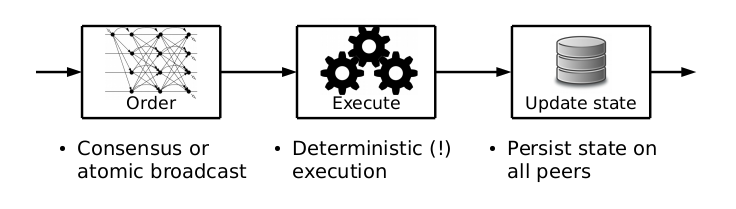
\includegraphics[width=0.8\linewidth]{imgs/orderExecuteArchitecture.png}
  \caption{\label{fig:orderexecute} Order-execute architecture in Replicated
  Services Like Ethereum (Source: IBM, 2018)}
\end{figure}

On the other hand, the order-execute architecture is conceptually simple,
leading it to be currently widely implemented in replicated services such as
Blockchain. In this architecture the transactions are executed sequentially on
all peers which limits the maximum number of simultaneous transactions that can
be achieved.  Additionally a Denial of Service attack can be mounted just by
deploying a slow performing smart contract or one with an infinite loop to the
network since the Blockchain forms a distributed computing engine.  To cope
with this issue, public programmable Blockchains with an associated
cryptocurrency, account for the execution cost of executing of the program.

In Fabric all nodes that participate in the network have an identity, as
provided by a modular Membership Service Provider (MSP).  A MSP is a component
that aims to offer the abstraction of a membership operation architecture
meaning that all identities are only allowed to participate if verified to be
considered trustworthy.  The MSP maintains the identities of all nodes in the
system and is responsible for issuing credentials that are used for node
authentication and authorization. A MSP may define their own notion of
identity, and the rules by which those identities are governed and
authenticated using signature generation and
verification~\cite{HyperledgerFabricDocs2017}.

Fabric also assigns different roles to peers. Nodes in Fabric network can have
one or more, of these three roles:

\begin{itemize}
  \item Clients submit transaction proposals for execution, help orchestrate
    the execution phase, and broadcast transactions for ordering.

  \item Peers execute transaction proposals and validate transactions.  All
    peers maintain the ledger, where all transactions  are recorded in the form
    of a hash chain, as well as the state, a succinct representation of the
    latest ledger state. Not all peers execute all transactions.

  \item Ordering Service Nodes or orderers are the nodes that collectively form
    the ordering service. In short, the ordering service establishes the total
    order of all transactions in Fabric, where each transaction contains state
    updates and dependencies computed during the execution phase, along with
    cryptographic signatures of the endorsing peers defined in the endorsing
    policy of the transaction. Orderers are entirely unaware of the application
    state, and do not participate in the execution nor in the validation of
    transactions. This design choice renders consensus in Fabric as modular as
    possible and simplifies the replacement of consensus protocols in Fabric. 
\end{itemize}

Looking ahead, Hyperledger Fabric will continue to focus on privacy and
confidentiality with v1.2 being recently released, v1.3 and 1.4 expected to be
out this year with further emphasis on these aspects in a regular quarterly
cadence~\cite{hyperledgerRoadmap2018}.

\section{An Overview of Blockchain Platforms}

In this section a brief comparison is made between the platforms introduced in
this Chapter. As seen in Table~\ref{tab:blockchainComparison}, different
Blockchain implementations have different characteristics and focus.

\begin{table}[h!]
	\centering
	
	\begin{tabular}{ p{4cm} p{3.4cm} p{4cm} p{4.4cm} }
    \textbf{Characteristics} & \textbf{Bitcoin} & \textbf{Ethereum} &
    \textbf{Fabric} \\ \hline
    Permission Restrictions & Permissionless & Permissionless & Permissioned
    \\[7pt] Access to Data & Public & Public or Private & Private \\[7pt]
    Consensus & Proof-of-Work & Proof-of-Work
    (\href{https://github.com/ethereum/wiki/wiki/Ethash}{Ethash}) & Practical
    Byzantine Fault Tolerant \\[7pt] Governance & Low, decentralized decision
    making by community/miners & Medium, core developer group, community
    improvement proposals & Low, open-governance model based on Linux model
    \\[7pt] Native Currency & Yes, Bitcoin & Yes, Ether & No \\[7pt] Scripting
    & Limited possibility & Turing-complete virtual machine, Solidity DSL
    language & Turing-complete scripting chaincode, multiple general purpose
    language support \\[7pt] Focus & Financial Transactions & General Purpose &
    Enterprise Focused \\
		\hline
	\end{tabular}
	
	\caption
	[Characteristics Comparison between Bitcoin, Ethereum and Fabric.]
	{Characteristics Comparison between Bitcoin, Ethereum and Fabric.}
	
	\label{tab:blockchainComparison}
\end{table}

